\chapter{Employing GPUs in scientific algorithms}

The information age has brought a massive increase in the amount of data that is being collected and processed. The `data explosion' can be observed in virtually every field of computer science. In the scientific domain, this phenomenon is multiplied by increasingly powerful data gathering devices (i.e., cytometers in bioinformatics, optic sensors in physics, seismometers in geology, etc.). The amount of data is simply too large to be processed in a required time using. To alleviate this apparent pressure, the corresponding algorithm (which typically have super-linear time complexity) must be ported to massively parallel architectures, such as GPUs. The provided advantage can in return be the ability to assess bigger data, use more detailed processing methods or to analyze the data in real time.

This chapter enumerates four selected scientific algorithms and discusses their challenges in porting to GPUs to enable higher performance.

\section{Hierarchical clustering with the Ma\-ha\-la\-no\-bis linkage}

In the field of bioinformatics, the hierarchical clustering is a popular method for analyzing various types of data. 
In general, hierarchical clustering is an unsupervised machine learning method that aims to group the data points into clusters according to some linkage criterion.
It is an iterative method that starts with each data point being a cluster and in each iteration merges the two most similar clusters according to the linkage criterion until there is only one cluster.
There are many cluster linkage criteria, each of them having its own advantages and disadvantages. 
The most common linkage is the \emph{centroid linkage} which computes the distance between the clusters centroids (the mean points).
In analyzing single-cell cytometry data, hierarchical clustering with the Mahalanobis linkage has been shown to be the most suitable method.

Mahalanobis linkage uses \emph{Mahalanobis distance} to measure the similarity between clusters:
\begin{defn}[Mahalanobis distance]
	Suppose a probability distribution $C$ on $\R^d$ with mean $\bar{C} \in \R^d$ and a convariance matrix $\cov(C)$. If the matrix $\cov(C)$ is regular, we define the \emph{Mahalanobis distance} between $u \in \R^d$ and $C$ as
	\begin{equation}
	d_\text{Maha}(u,C) = \sqrt{(u-\bar{C})^T\cov(C)^{-1}(u-\bar{C})}.
	\end{equation}\label{eq01:maha}
\end{defn}

If we generalize a centroid of a cluster to a probability distribution, Definition~\ref{eq01:maha} can be used to define the Mahalanobis distance between a point and a cluster. To extend the definition to a distance between two clusters, we use the following equation:
\begin{equation}
    \delta_\text{Maha}(P,Q) = \frac{d_\text{Maha}(\bar{P},Q) + d_\text{Maha}(\bar{Q},P)}{2}
\end{equation}\label{eq01:maha_linkage}

To illustrate the measure of the Mahalanobis distance, let us suppose we have two elliptic clusters. In the means of the proximity, the measure favors such clusters that their ellipsis are alongside rather than in a prolongation of one another [TODO] (see Figure~\ref{fig:ellipses}). 
Only when the objects of a cluster form a spherical shape, this measure of dissimilarity is proportional to the euclidean distance with a corresponding linkage.
This allows for a very natural formation of clusters in biological data. However, the benefits come with the increase in complexity materialized in the computation of covariance matrix, matrix inverse and vector-matrix-vector multiplication in each distance evaluation.

\begin{figure}[h]
    \centering
    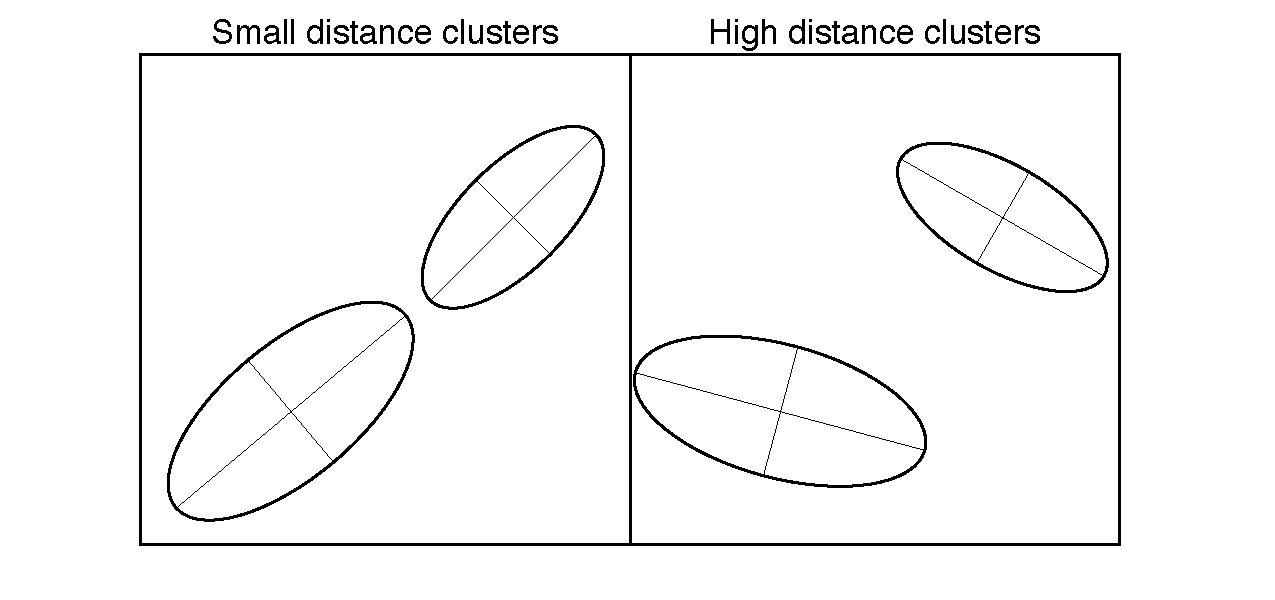
\includegraphics[width=0.6\textwidth]{img/ellipses.pdf}
    \caption{Two pairs of clusters with different simillarities according to Mahalanobis distance}
    \label{fig:ellipses}
\end{figure}

% where P is the set mean and cov(P) is the covariance matrix of the set P (if interpreted as a `distribution of points').
% The distance has a specific property which can be intuitevely interpreted as a Euclidean distance to a center of a set which `accounts' the shape and size of the cluster. In other words, the Mahalanobis distance is a Euclidean distance in a transformed space, such that the covariance matrix of a cluster is the identity matrix.

% In the Mahalanobis linkage, the distance between two clusters is defined as the average of Mahalanobis distances between their means and each other.
% This allows for a very natural formation of clusters in biological data. However, the benefits come with the increase in complexity. 
% To compute the Mahalanobis distance, we need to compute the mean of a cluster and an inverse of its covariance matrix and finally do an actual distance computation which are two matrix multiplications.

\subsection{Algorithm complexity and the implementation}

Hierarchical Clustering (HC) is a well known problem and there are many algorithms which effectively solve it. Roughly, they can be divided into categories according to the data structures they employ [TODO]:
\begin{itemize}
    \item HC with a dissimilarity matrix --- the most straightforward approach; the dissimilarity matrix stores the distances between all pairs of clusters. This approach has a cubic time complexity and quadratic memory complexity.
    \item HC with a nearest neighbor array --- each cluster stores the index of its nearest neighbor. This approach trades a linear memory complexity for an asymptotic time complexity of $\mathcal{O}(d \cdot n^3)$.
    \item HC with an array of priority queues --- a more sophisticated solution, which reduces the time complexity to $\mathcal{O}(n^2 \log n)$.
\end{itemize}

C application \texttt{mhclust}, the original implementation of the Mahalanobis HC, uses the dissimilarity matrix. This approach is simple and allows for a straightforward implementation. However, the empirical data reveal the biggest limiting factor in the quadratic memory complexity. This is supported more by the fact that GPU memory is typically limited to a few gigabytes. Therefore, we decided to use the nearest neighbor array approach. This approach has a hidden benefit --- if a number of neighbors to update in an iteration is constant $u$, the time complexity of the algorithm is reduced to $\mathcal{O}(d \cdot n^2 \cdot u)$. This is also supported by the evaluation on real data, where the number of neighbors to update is typically in the range of 10 to 100. 

- maybe better start with DM and PQ - describe the costly parts of the loop with DM and show optimizations with PQ
- then, start with memory limitations in the original impl
- then, propose in-place distance computation and optimization of the nearest neighbor arrays and neighbor buffering
- then, show the results ? - how bigger the data can be assuming X GB of memory

- future work: tensor cores, cuda graph


\subsection{Prior solution and its limitations}

High computational complexity limited the original implementation of the algorithm to a maximum thousands of dataset points. To overcome this limitation, the authors developed the method of apriori clusters to reduce the dataset size for the sake of the accuracy. The apriori clustering is a preprocessing step in which small clusters are created using Euclidean distance. Then these clusters are inputed to the main algorithm. This allowed to push the limits of the original implementation in orders of magnitude, but at a cost of less accurate results.

The memory complexity is also a limiting factor. The original implementation uses a dissimilarity matrix to store the distances between the clusters. Although this data structures saves computation time (in distance evaluation), it has quadratic memory complexity. This limits the size of the dataset to a few thousands of points.

\subsection{Optimized solution}

In our solution, we use a nearest neighbor array instead of the dissimilarity matrix. This allows us to reduce the memory complexity to linear. The nearest neighbor array is a one-dimensional array of size $n$ where $n$ is the number of clusters. Each element of the array contains the index of the nearest neighbor of the corresponding cluster. Although it requires more updates in the worst case, we used a simple optimization to buffer multiple nearest neighbors for each cluster.

The other challenge was that the complete solution was composed of multiple kernels of different duration. The computation of covariance matrix is fast at the beginning of the algorithm (because the clusters are small) while nearest neighbor list updates are slow (because there are more potential neighbors to update). Thankfully, these two kernels are independent and can be executed in parallel. We used CUDA streams to overlap the execution of these two kernels and thus keeping the high utilization of the GPU.

\section{Neighborhood-based dimensionality reduction}

EmbedSOM is a dimensionality reduction tool based on self-organizing maps (SOM). It competes with other dimensionality reduction tools such as t-SNE or UMAP giving the advantage of better computational complexity which favors it as a semi-supervised real-time dataset analytic tool while retaining the competitive accuracy of the results.
Although achieving a good performance, a true real time visualisation on big datasets was lacking. 

In the landmark based dimensionality reduction method, high dimensional data points are mapped to lower-dimensonal space according to the location to a set of landmarks, which have low-dimensional counterparts.
The EmbedSOM algorithm encompasses the following steps for each point:
\begin{enumerate}
    \item A set of $k$ nearest landmarks is found and scored according to the distance to the point.
    \item For each pair of the nearest landmarks (u,v), do the orthogonal projection of the point to the line between the landmarks and select the suitable low-dimensional mapping.
\end{enumerate}

The challenges of this algorithm is the low arithmetic intensity in both steps - generally, we want to execute the most operations on read data but if taken naively, each acessed data point would be presented with just one operation (either euclidean projection or distance computation).
There are two approaches on dealing with this problem - either design a smart caching of read data so it is used in multiple operations or design a kernel with high thread occupancy so the latency of retriving the data is hidden by scheduling multiple threads.

We used both approaches in our implementation. The kNN step is implemented using bitonic sort, which promotes the overlapping of data with computation. In the projection step, each thread loads multiple landmarks into registers such that it can perform multiple ortogonal projections in parallel. This approach is similar to the one used in the Mahalanobis linkage.

optimizations:

memory-heavy stuff:
- using registers as caches
- vector loads

\section{Cross-correlation}

Cross-correlation is a method for finding the similarity of two signals. It is used in many fields of science, such as image processing, seismology, bioinformatics, etc. For discrete 1D signals, the cross-correlation is defined as
$$ \sum_{i=0}^{n-1} x_i y_{i + \tau} $$
where $x$ and $y$ are the signals and $\tau$ is the shift of the second signal. The cross-correlation is usually computed for all possible shifts. Depending on the application, the maximum or minimum of the cross-correlation is used as a measure of similarity.
We devoted our attention to the cross-correlation of 2D signals, which can be defined as a sum of element-wise products of all the overlaps between the two signals. The cross-correlation of two 2D signals is therefore a 2D matrix.

This problem combines the challenges from the previous examples. Specifically, we have
\begin{itemize}
    \item poor load balancing - the computation of each element of the output matrix takes a different amount of time
    \item low arithmetic intensity - the computation of each element of the output matrix requires a small amount of arithmetic operations
\end{itemize}

The solution for the first problem could be a dynamic parallelism. However, the problem size, which we paid our attention to, was too small to justify the overhead of dynamic parallelism. Therefore, we had to come up with a different solution of smart work distribution.

For the second problem, we evvaluated different approaches of data caching in registers.

In the result, we achieved a better performance than the asymtotically better methods (such as FFT-based cross-correlation) for small problem sizes.

\section{Stochastic simulation of Boolean networks}

definition of stochastic simulation

limitations of real time processing

runtime compilation and linkage of model code